\subsubsection{\stid{2.11} BOLT: Lightning Fast OpenMP}\label{subsubsect:bolt}

\paragraph{Overview}

OpenMP is central for several applications that target Exascale,
including ECP applications, to exploit on-node computational
resources.  Unfortunately, current production OpenMP runtimes, such as
those that ship with Intel and GNU compilers, are inadequate for the
massive and fine-grained concurrency expected at the Exascale level.
These runtimes rely on heavy-handed OS-level threading strategies that
incur significant overheads at fine-grained levels and exacerbate
interoperability issues between OpenMP and internode programming
systems, such as MPI and OpenSHMEM.  Our solution is a production
quality OpenMP runtime (called BOLT) that leverages user-level threads
instead of OS-level threads (e.g., Pthreads).  Due to their
lightweight nature, managing and scheduling user-level threads incurs
significantly less overhead.  Furthermore, interoperability between
BOLT and internode programming systems opens up new optimization
opportunities by promoting asynchrony and reducing hardware
synchronization (atomics and memory barriers).  Initial studies on
this proposal can be found in \cite{amer2018, ccgrid, ppopp}. This report
briefly summarizes the issues in OpenMP runtimes that rely on OS-level
threading, describes BOLT as the solution to this challenge, the
current status in the BOLT effort, and the next steps for further
improvements.

\paragraph{Key Challenges}

The growing hardware concurrency in High Performance Computing (HPC)
cluster nodes is pushing applications to chunk work more fine-grained
to expose parallelism opportunities.  This is often achieved through
nested parallelism either in the form of parallel regions or explicit
tasks.  Nesting parallel regions can potentially cause
oversubscription of OS-level threads to CPUs and thus lead to
expensive OS-level thread management.  Such heavy costs usually
outweigh the benefits of increased concurrency and thus compels the
OpenMP programmer to avoid nested parallel regions altogether.  Such
workaround, however, not only causes poor resource utilization from
insufficient parallelism but is also not always possible.  For
instance, the nested level could be outside the control of the user
because it belongs to an external library that also uses OpenMP
internally.  Internode programming systems, such as MPI and OpenSHMEM,
are not aware of OpenMP semantics, such as the notion of an OpenMP
task.  What these internode systems understand is the low-level
threading layer used by OpenMP, such as Pthreads.  This threading
layer serves as the interoperability medium between OpenMP and the
internode programming system and has a direct impact on performance.
For instance, when OpenMP threads are allowed to concurrently perform
internode communication, the interoperability layer dictates how
thread safety and progress on communication is handled.  It is
notoriously known that OS-level thread safety in production MPI
libraries suffers significant performance issues.  Despite the recent
improvements to OS-level thread safety in MPI libraries, the
state-of-the-art performance results are still indicating serious
scalability issues.  While continued progress on improving OS-level
thread safety in these important internode programming systems is
crucial for traditional interoperability, we propose in this work
exploring an orthogonal direction that assumes a more lightweight
interoperability layer.

\paragraph{Solution Strategy}

Both fine-grained parallelism and interoperability issues suffer from
the heavy nature of working at the level of OS threads.  Our solution
to both challenges leverages user-level threads.  Using user-level
threads as the underlying threading layer for the OpenMP runtime
offers a significantly better trade-off between high concurrency and
thread management overheads.  This allows users to generate
fine-grained concurrency and oversubscription without worrying about
the performance collapse that is observed in current OpenMP runtimes.
Our OpenMP runtime, BOLT, is derived from the LLVM OpenMP runtime and
leverages Argobots, a highly optimized lightweight threading library,
as its underlying threading layer.  OpenMP threads and tasks are
spawned as Argobots work units and nested parallel regions are managed
through an efficient work-stealing scheduler.  Furthermore, new
compiler hints and runtime optimizations have been developed to allow
reducing thread management overheads even further~\cite{iwasaki2018}.
Interoperability improvements have also been demonstrated by having
BOLT interoperate with an MPI library (MPICH) through the Argobots
threading layer rather than OS-level threads.  Results showed that
this approach allows better communication progress and outperforms the
traditional Pthreads-level interaction~\cite{seo2018}.

\paragraph{Recent Progress}

The development of BOLT went through several steps that involved
developing or optimizing various aspects.  The first step was to fork
BOLT from the upstream LLVM OpenMP runtime (https://openmp.llvm.org)
and replace the Pthreads layer with a basic Argobots design. As shown
in Figure~\ref{fig:sollve-bolt}, BOLT takes advantage of the maturity
and the ABI compatibility of the LLVM OpenMP runtime with the Intel
and GCC compilers, which makes it easily deployable in production
environments.  Next, we implemented advanced scheduling strategies to
improve the performance of BOLT under fine-grained nested parallelism
regimes.  The following step was to investigate ways to reduce thread
management overheads by exploiting application knowledge.  By taking
into account the suspension likelihood of a thread or task (e.g.,
yield execution on a blocking I/O operation), we have extended
Argobots to leverage such information, incorporated these features
into the BOLT runtime, and developed prototype compiler hints to
exploit them. With respect to interoperability with MPI, we have
investigated the shortcomings of current interoperability models at
the implementation as well as standard specification levels.  We have
investigated the benefits of having a more lightweight
interoperability layer through Argobots using BOLT as the OpenMP
runtime and MPICH as the MPI library and demonstrated encouraging
results.

BOLT and Argobots have been subject to three releases and the
associated scientific contributions have been published in top tier
venues in the field.  The latest BOLT release has been upgraded to be
compatible with LLVM OpenMP 7.0, which includes support for the
important explicit task dependency and task loop features, and has
been subject to more optimizations and validation testing. More
applications that could benefit from BOLT within and outside ECP have
been discovered and BOLT's position within the ECP ecosystem has been
solidified through new connections with other software technology and
application projects.

\begin{figure}[htb]
  \centering
  \vspace{2.0ex}
  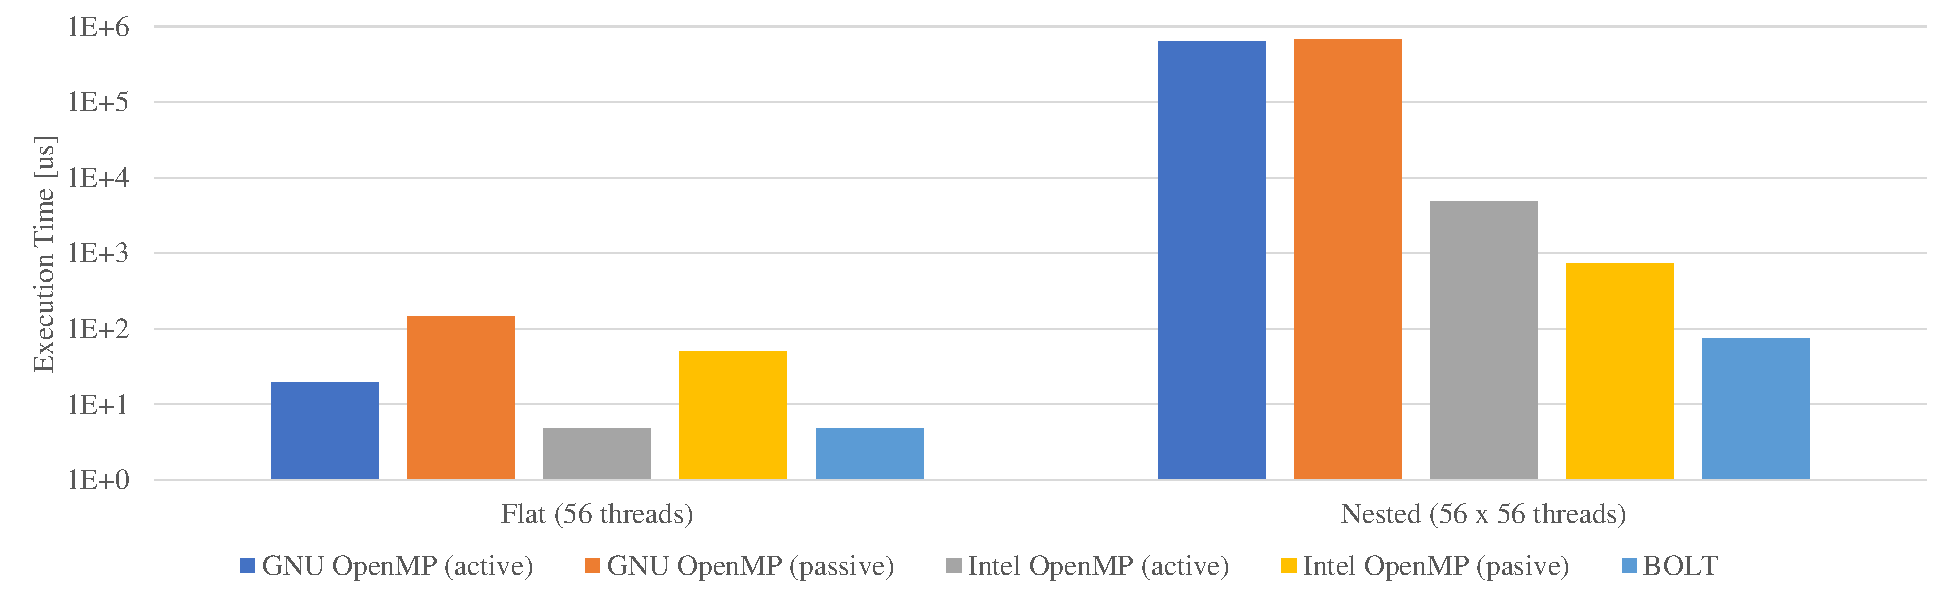
\includegraphics[width=0.9\columnwidth]{projects/2.3.2-Tools/2.3.2.11-SOLLVE/SOLLVE-BOLT.pdf}
  \caption{\label{fig:sollve-bolt}Pictorial representation of development of BOLT}
  \vspace{2.0ex}
\end{figure}

\paragraph{Next Steps}

Some aspects of BOLT require further work and investigation.  In the
following we enumerate some of the key aspects under progress:

\begin{enumerate}

\item Tighter integration of BOLT with the other components of the
SOLLVE project

\item Despite BOLT has reached more applications and users, its reach
and impact remain limited.  We plan to investigate a wider range of
applications, including ECP ones, and expand the BOLT user base.  This
will allow us to evaluate the effectiveness of our solution and
potentially discover new areas of needed improvement as well as
increase BOLT's impact among users.

\item The interoperability results between BOLT and MPI were
  encouraging but still preliminary.  We are planning on doing more
  extensive evaluation of this interoperability layer with benchmarks
  and applications and potentially implement improvement if
  scalability is unsatisfactory.

\item Finally, we plan to perform more rigorous robustness testing
  with validation and test suites as well as with fully-fledged
  applications and proxy-application for as much coverage as possible.

\end{enumerate}
